\documentclass{article}
\usepackage{tikz}
\usetikzlibrary{decorations.markings}
\usepackage{xcolor}

\title{Pictures}
\author{Alwyn Bakker}

\begin{document}

\tikzset{->-/.style={decoration={markings, mark=at position #1 with {\arrow[scale=1.5]{>}}}, postaction={decorate}}} %sets up style for arrows partway along lines
\tikzset{-<-/.style={decoration={markings, mark=at position #1 with {\arrow[scale=1.5]{<}}}, postaction={decorate}}}


\begin{figure}
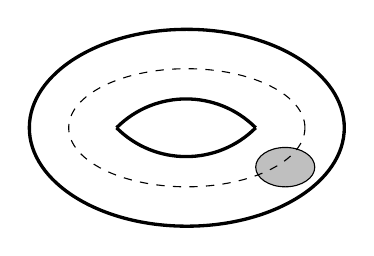
\begin{tikzpicture} [scale=0.5] %punctured torus
\def \torus{(0,0) ellipse (4 and 2.5) (1.75,0) arc [radius=2.5, start angle=45, end angle=135] (1.75,0) arc [radius=2.5, start angle=315, end angle=225]};
\draw [very thick] \torus;
\filldraw[fill=lightgray, thin] (2.5,-1) ellipse (0.75 and 0.5);
\draw[dashed] (0,0) ellipse (3 and 1.5);
\end{tikzpicture}
\caption{A punctured torus.}
\end{figure}

\begin{figure}
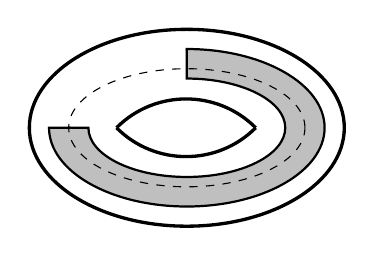
\begin{tikzpicture} [scale=0.5] %deform point one
\filldraw[thick, fill=lightgray] (2.5,0) -- (1.5,0) arc [start angle=-180, end angle=90, x radius=3.5, y radius=2] -- (5,1.25);
\filldraw[thick, fill=white] (2,0) -- (2.5,0) arc [start angle=-180, end angle=90, x radius =2.5, y radius = 1.25] -- (5,2);
\draw[very thick] (5,0) ellipse (4 and 2.5);
\draw[dashed] (5,0) ellipse (3 and 1.5);
\draw[very thick] (6.75,0) arc [radius=2.5, start angle=45, end angle=135];
\draw[very thick] (6.75,0) arc [radius=2.5, start angle=315, end angle=225];
\end{tikzpicture}
\caption{Deforming the puncture.}
\end{figure}


\begin{figure}
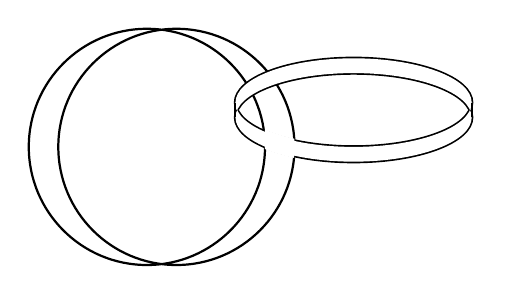
\begin{tikzpicture} [scale=0.75] %connected bands
\def \bandh{(1,0.5) ellipse (2 and 0.75) (1,0.75) ellipse (2 and 0.75)}
\def \bandv{(-2.5,0) ellipse (2 and 2) (-2,0) ellipse (2 and 2)}

	%adds coordinates for tiny lines to make horizontal band look more bandy
\coordinate (htopl) at (-1.01,0.75);
\coordinate (hmidl) at (-1.01,0.625);
\coordinate (hbotl) at (-1.01,0.5);
\coordinate (htopr) at (3.01,0.75);
\coordinate (hmidr) at (3.01,0.625);
\coordinate (hbotr) at (3.01,0.5);
	%end of coordinate code
	
\draw [thick] \bandv;
\draw [very thick] \bandh;

\begin{scope}[even odd rule]
\fill [white] \bandh;
\clip (-0.5,-0.5) -- (-0.5,0.5) -- (0.5,0.5) -- (0.5,-0.5) -- cycle;
\clip \bandv;
\filldraw [ultra thick, color=white, fill=white] \bandh;
\end{scope}

\begin{scope} [even odd rule]
\clip (-1.25,1) -- (-1.25,0.625) -- (-0.98,0.625) -- (-0.95,1) -- cycle;
\fill [fill=white] (htopl) -- (hmidl) -- (1,0.5) ellipse (2 and 0.75) -- cycle;
\end{scope}

\begin{scope} [even odd rule]
\clip (3.25,1) -- (3.25,0.625) -- (2.98,0.625) -- (2.95,1) -- cycle;
\fill [fill=white] (htopr) -- (hmidr) -- (1,0.5) ellipse (2 and 0.75) -- cycle;
\end{scope}

	%draw tiny lines code
\draw [thick] (htopl) -- (hbotl);
\draw [thick] (htopr) -- (hbotr);

\end{tikzpicture}
\caption{The torus with puncture maximally deformed.}
\end{figure}



\begin{figure}
\begin{tikzpicture} %using shorten code to produce gaps
\coordinate (top) at (0,2);
\coordinate (mid) at (0,0);
\coordinate (bot) at (0,-2);

\draw [thick, shorten <= 5, shorten >= 5] (mid) to [out=120, in=-140] (top) to [out=40, in=-30, distance=100] (bot);
\draw [thick, shorten <=5, shorten >= 5] (bot) to [out=150, in=-120] (mid) to [out=60, in=-30] (top);
\draw [thick, shorten <=5, shorten >=5] (top) to [out=150, in =-150, distance=100] (bot) to [out=30, in=-40] (mid);
\end{tikzpicture}
\caption{The trefoil knot.}
\end{figure}

\begin{figure}
\begin{tikzpicture} %as trefoil but with orientation
\coordinate (top) at (0,2);
\coordinate (mid) at (0,0);
\coordinate (bot) at (0,-2);

\draw [thick, shorten <= 5, shorten >= 5, -<-=0.13, -<-=0.5] (mid) to [out=120, in=-140] (top) to [out=40, in=-30, distance=100] (bot);
\draw [thick, shorten <=5, shorten >= 5, -<-=0.3, -<-=0.8] (bot) to [out=150, in=-120] (mid) to [out=60, in=-30] (top);
\draw [thick, shorten <=5, shorten >=5, -<-=0.3, -<-=0.9] (top) to [out=150, in =-150, distance=100] (bot) to [out=30, in=-40] (mid);
\end{tikzpicture}
\caption{The trefoil knot with orientation.}
\end{figure}


\begin{figure}
\begin{tikzpicture} %trefoil with eliminated crossings

\coordinate (topl) at (0,2);
\coordinate (midl) at (0,0);
\coordinate (botl) at (0,-2);
\coordinate (topr) at (0.25, 2);
\coordinate (midr) at (0.25,0);
\coordinate (botr) at (0.25,-2);

\draw [thick, -<-=0.45] (midl) to [out=120, in=-140] (topl) to [out=150, in =-150, distance=100] (botl) to [out=150, in=-120] (midl);
\draw [thick, -<-=0.45] (midr) to [out=60, in=-30] (topr) to [out=40, in=-30, distance=100] (botr) to [out=30, in=-40] (midr);

\end{tikzpicture}
\caption{Eliminating the crossings in the oriented trefoil knot.}
\end{figure}

\begin{figure}
\begin{tikzpicture} %the trefoil as discs with twisted bands

%central coordinates
\coordinate (mid) at (0,0); \coordinate (top) at (0,1.5); \coordinate (bot) at (0,-1.5);

%left coordinates
\coordinate (topl1) at (-1,1.75); \coordinate (botl1) at (-1,1.25); \coordinate (topl2) at (-1,0.25); \coordinate (botl2) at (-1,-0.25); \coordinate (topl3) at (-1,-1.25); \coordinate (botl3) at (-1,-1.75);

%right coordinates
\coordinate (topr1) at (1,1.75); \coordinate (botr1) at (1,1.25); \coordinate (topr2) at (1,0.25); \coordinate (botr2) at (1,-0.25); \coordinate (topr3) at (1,-1.25); \coordinate (botr3) at (1,-1.75);

%top band
\draw [thick, ->-=0.3, ->-=0.8] (topr1) to [out=180, in=45] (top) to [out=-135, in=0] (botl1);
\draw [thick, shorten >=5,  -<-=0.5] (botr1) to [out=180, in =-45] (top);
\draw [thick, shorten <=5,  -<-=0.5] (top) to [out=135, in=0] (topl1);

%mid band
\draw [thick, ->-=0.3, ->-=0.8] (topr2) to [out=180, in=45] (mid) to [out=-135, in=0] (botl2);
\draw [thick, shorten >=5, -<-=0.5] (botr2) to [out=180, in =-45] (mid);
\draw [thick, shorten <=5,  -<-=0.5] (mid) to [out=135, in=0] (topl2);

%bot band
\draw [thick, ->-=0.3, ->-=0.8] (topr3) to [out=180, in=45] (bot) to [out=-135, in=0] (botl3);
\draw [thick, shorten >=5,  -<-=0.5] (botr3) to [out=180, in =-45] (bot);
\draw [thick, shorten <=5,  -<-=0.5] (bot) to [out=135, in=0] (topl3);

%left disc
\draw [thick] (topl3) to [out=85, in=-85] (botl2);
\draw [thick] (topl2) to [out=85, in=-85] (botl1);
\draw [thick, -<-=0.4] (topl1) to [out=125, in=-125, distance=100] (botl3);

%right disc
\draw [thick] (topr3) to [out=95, in=-95] (botr2);
\draw [thick] (topr2) to [out=95, in=-95] (botr1);
\draw [thick, -<-=0.4] (topr1) to [out=55, in=-55, distance=100] (botr3);

\end{tikzpicture}
\caption{Seifert surface as discs connected with twisted bands. Note the boundary of the surface is the oriented trefoil knot.}
\end{figure}


\begin{figure}
\begin{tikzpicture}
%central coordinates
\coordinate (top) at (0,1.5); \coordinate (bot) at (0,-1.5);
%left coordinates
\coordinate (topl1) at (-1,1.75); \coordinate (botl1) at (-1,1.25); \coordinate (topl3) at (-1,-1.25); \coordinate (botl3) at (-1,-1.75);
%right coordinates
\coordinate (topr1) at (1,1.75); \coordinate (botr1) at (1,1.25); \coordinate (topr2) at (1,0.25); \coordinate (botr2) at (1,-0.25); \coordinate (topr3) at (1,-1.25); \coordinate (botr3) at (1,-1.75);

%far right coordinates
\coordinate (twistfr) at (5,1.75); \coordinate (twistfr+) at (5.1,2.15);
\coordinate (topfr) at (4,0.5); \coordinate (botfr) at (4,-0.5);

%extra mid band coordinates
\coordinate (extopr) at (1,0.5); \coordinate (exbotr) at (1,0); \coordinate (extopl) at (2.35,1.4); \coordinate (exbotl) at (2.4, 1); \coordinate (extopm) at (2.4, -1); \coordinate (exbotm) at (2.35,-1.4);
\coordinate (exbotr-) at (0.95,-.15); \coordinate (topr2-) at (0.95,0.3);

%top band
\draw [thick, ->-=0.3, ->-=0.8] (topr1) to [out=180, in=45] (top) to [out=-135, in=0] (botl1);
\draw [thick, shorten >=5,  -<-=0.5] (botr1) to [out=180, in =-45] (top);
\draw [thick, shorten <=5,  -<-=0.5] (top) to [out=135, in=0] (topl1);
%bot band
\draw [thick, ->-=0.3, ->-=0.8] (topr3) to [out=180, in=45] (bot) to [out=-135, in=0] (botl3);
\draw [thick, shorten >=5,  -<-=0.5] (botr3) to [out=180, in =-45] (bot);
\draw [thick, shorten <=5,  -<-=0.5] (bot) to [out=135, in=0] (topl3);

%mid band
\draw [thick] (botr2) to [out=180, in=-125] (exbotr);
\draw [thick, -<-=0.6] (exbotr) to [out=55, in=-155] (exbotl);
\draw [thick, shorten >=3, -<-=0.2, -<-=0.7] (exbotl) to [out=25, in=-170] (twistfr) to [out=10, in=45, distance=25] (topfr) to [out=-125, in=125] (botfr);
\draw[thick, shorten <=3, -<-=0.5] (botfr) to [out=-45, in=0] (exbotm);

\draw [thick] (topr2-) to [out=92, in=-125] (extopr);
\draw [thick, ->-=0.5] (extopr) to [out=55, in=-155] (extopl);
\draw [thick, ->-=0.5] (extopl) to [out=25, in=-175] (twistfr+);
\draw [thick, shorten >=3, shorten <=3, ->-=0.5] (twistfr) to [out=-135, in=135] (topfr);
\draw [thick, shorten <=3, ->-=0.7] (topfr) to [out=-30, in=55] (botfr) to [out=-135, in=0] (extopm);

\draw [thin] (twistfr+) to [out=0, in=90] (5.3,1.73);

%left disc
\draw [thick] (topl3) to [out=85, in=-85] (botl1);
\draw [thick, -<-=0.4] (topl1) to [out=125, in=-125, distance=100] (botl3);

%right disc
\draw [thick] (topr3) to [out=95, in=-95] (botr2);
\draw [thin] (exbotr-) to [out=92, in=-92] (topr2-);
\draw [thick] (extopr) to [out=95, in=-95] (botr1);
\draw [thick, shorten >=2] (topr1) to [out=55, in=105, distance=25] (extopl);
\draw [thick, shorten <=2] (exbotl) to [out=-87, in=87] (extopm);
\draw [thick] (exbotm) to [out=-105, in=-55, distance=25] (botr3);
\end{tikzpicture}
\caption{Deforming the surface by sliding one end of the central band onto the same disc as its opposite end. Note the central band collects an extra half-twist as it slides around the edge of the top band.}
\end{figure}



\begin{figure}
\begin{tikzpicture}
%central connection coords
\coordinate (topl) at (-0.25,0.25); \coordinate (topr) at (0.25, 0.25);, \coordinate (botl) at (-0.25, -0.25); \coordinate (botr) at (0.25,-0.25);

%horizontal band coords
\coordinate (htopl) at (-1.25,0.5); \coordinate (hbotl) at (-1.25,0); \coordinate (hmidl) at (-1.25, 0);
\coordinate (hmidtl) at (-0.25,1.3); \coordinate (hmidbl) at (-0.25, 0.8);
\coordinate (hmidtr) at (0.25, 1.5); \coordinate (hmidbr) at (0.25, 1);
\coordinate (hlefttop) at (3.1,3); \coordinate (hlefttopl) at (3.35, 2.7);
\coordinate (hrighttop) at (3.05,2.65); \coordinate (hrighttopm) at (2.9,1.6); \coordinate (hrighttopb) at (2.9,0.5);
\coordinate (hextra) at (3.4,2.6);

%vertical band coords
\coordinate (vtopl) at (-0.25,3); \coordinate (vtopr) at (0.25, 2.8); \coordinate (vtopm) at (-0.08,2.6);
\coordinate (vcrosst) at (-2.5, 1.5); \coordinate (vcrossb) at (-2.5,0);
\coordinate (vbotl) at (-0.25, -2.5); \coordinate (vbotr) at (0.25,-2.3); \coordinate (vbotm) at (-0.1, -2.1);

%horizontal band draw
\draw [thick, shorten >=7, ->-=0.5] (topl) to [out=180, in=-80] (htopl);
\draw [thick, distance=19, ->-=0.7] (hmidl) to [out=95, in=-160] (hmidtl);
\draw [thick, ->-=0.5] (hmidtl) to [out=20,in=-160] (hmidtr) to [out=20, in=-170] (hlefttop);
\draw [thin] (hlefttop)  to [out=-10, in=90] (hextra);

\draw [thick, -<-=0.2, -<-=0.8] (botl) to [out=180, in=-85] (hbotl) to [out=95, in=-160] (hmidbl);
\draw [thick, distance=10, -<-=0.5] (hmidbl) to [out=20, in=-160] (hmidbr) to [out=20, in=160] (hlefttopl);

\draw [thick, shorten >=2, ->-=0.5] (hrighttop) to [out =-100, in=135] (hrighttopm);
\draw [thick, shorten <=2, distance=15, ->-=0.2, ->-=0.65] (hrighttopm) to [out=-45, in=45] (hrighttopb) to [out=-135, in=0] (topr);
\draw [thick, shorten >=2, distance=10, -<-=0.3, -<-=0.8] (hlefttopl) to [out=-60, in=45] (hrighttopm) to [out=-135, in=135] (hrighttopb);
\draw [thick, shorten <=2, distance=30, -<-=0.55] (hrighttopb) to [out=-45, in=0] (botr);

%vertical band draw
\draw [thick, shorten >=2, -<-=0.5] (topl) to [out=90,in=-90] (hmidbl); \draw [thick, shorten >=2, ->-=0.5] (topr) to [out=90, in=-90] (hmidbr);
\draw [thick, shorten <=2, distance=12, -<-=0.5] (hmidtl) to [out=90, in=0] (vtopl);
\draw [thick, shorten <=2, distance=11, ->-=0.5] (hmidtr) to [out=90, in=-40] (vtopr);
\draw [thin] (vtopr) to [out=140, in=0] (vtopl);

\draw [thick, distance=13, shorten >=2, ->-=0.35, ->-=0.8] (vtopm) to [out=180, in=45] (vcrosst) to [out=-135,in=135] (vcrossb);
\draw [thick, shorten >=2, distance=22, -<-=0.5] (vtopl) to [out=180, in=135] (vcrosst);
\draw [thick, shorten <=2, -<-=0.5] (vcrosst) to [out=-45, in=45] (vcrossb);
\draw [thick, distance=25, -<-=0.5] (vcrossb) to [out=-135, in=180] (vbotl);
\draw [thick, shorten <=2, distance=25, ->-=0.5] (vcrossb) to [out=-45,in=180] (vbotm);
\draw [thick, distance=10, -<-=0.5] (vbotl) to [out=0, in=-90] (botl);
\draw [thick, distance=10, ->-=0.5] (vbotr) to [out=30, in=-90] (botr);
\draw [thin] (vbotl) to [out=0, in=-150] (vbotr);  %%for whatever reason, this isn't drawing...
\end{tikzpicture}
\caption{Shrinking both discs down results in two connected bands with two half-twists in each.}
\end{figure}

%\begin{tikzpicture}
%%central connection coords
%\coordinate (topl) at (-0.25,0.25); \coordinate (topr) at (0.25, 0.25);, \coordinate (botl) at (-0.25, -0.25); \coordinate (botr) at (0.25,-0.25);
%%horizontal band coords
%\coordinate (htopl) at (-1.25,0.25); \coordinate (hbotl) at (-1.2,0.1); \coordinate (hmidl) at (-1.25, 0);
%\coordinate (hmidtl) at (-0.25,1.3); \coordinate (hmidbl) at (-0.25, 0.8);
%\coordinate (hmidtr) at (0.25, 1.5); \coordinate (hmidbr) at (0.25, 1);
%\coordinate (hlefttop) at (3.05,3); \coordinate (hlefttopl) at (3.35, 2.7);
%\coordinate (hrighttop) at (3.05,2.65); \coordinate (hrighttopm) at (2.9,1.6); \coordinate (hrighttopb) at (2.9,0.5);
%\coordinate (hextra) at (3.4,2.6);
%%vertical band coords
%\coordinate (vtopl) at (-0.25,3); \coordinate (vtopr) at (0.25, 2.5); \coordinate (vtopm) at (-0.08,2.6);
%\coordinate (vcrosst) at (-2.5, 1.5); \coordinate (vcrossb) at (-2.5,0);
%\coordinate (vbotl) at (-0.25, -2.5); \coordinate (vbotr) at (0.2,-2); \coordinate (vbotm) at (-0.1, -2.1);
%%horizontal band draw
%\draw [thick, shorten >=3, ->-=0.5] (topl) to [out=180, in=-10] (htopl);
%\draw [thick, shorten <=1, distance=20, ->-=0.7] (htopl) to [out=170, in=-160] (hmidtl);
%\draw [thick, ->-=0.5, shorten >=2] (hmidtl) to [out=20,in=-160] (hmidtr) to [out=20, in=-170] (hlefttop) to [out=10, in=45] (hrighttop);
%
%\draw [thick, -<-=0.2, -<-=0.8] (botl) to [out=180, in=-70] (hbotl) to [out=110, in=-160] (hmidbl);
%\draw [thick, distance=10, -<-=0.5] (hmidbl) to [out=20, in=-160] (hmidbr) to [out=20, in=160] (hlefttopl);
%
%\draw [thick, shorten <=2, shorten >=2, ->-=0.5] (hrighttop) to [out =-100, in=135] (hrighttopm);
%\draw [thick, shorten <=2, distance=15, ->-=0.2, ->-=0.65] (hrighttopm) to [out=-45, in=45] (hrighttopb) to [out=-135, in=0] (topr);
%\draw [thick, shorten >=2, distance=10, -<-=0.3, -<-=0.8] (hlefttopl) to [out=-60, in=45] (hrighttopm) to [out=-135, in=135] (hrighttopb);
%\draw [thick, shorten <=2, distance=30, -<-=0.55] (hrighttopb) to [out=-45, in=0] (botr);
%%vertical band draw
%\draw [thick, shorten >=2, -<-=0.5] (topl) to [out=90,in=-90] (hmidbl); \draw [thick, shorten >=2, ->-=0.5] (topr) to [out=90, in=-90] (hmidbr);
%\draw [thick, shorten <=2, distance=12, -<-=0.5] (hmidtl) to [out=90, in=0] (vtopl);
%\draw [thick, shorten <=2, shorten >=2, ->-=0.5] (hmidtr) to [out=90, in=-45] (vtopr) to [out=135, in=0] (vtopm);
%
%\draw [thick, distance=13, shorten <=2, shorten >=2, ->-=0.35, ->-=0.8] (vtopm) to [out=180, in=45] (vcrosst) to [out=-135,in=135] (vcrossb);
%\draw [thick, shorten >=2, distance=22, -<-=0.5] (vtopl) to [out=180, in=135] (vcrosst);
%\draw [thick, shorten <=2, -<-=0.5] (vcrosst) to [out=-45, in=45] (vcrossb);
%\draw [thick, distance=25, -<-=0.5] (vcrossb) to [out=-135, in=180] (vbotl);
%\draw [thick, shorten <=2, shorten >=2, distance=25, ->-=0.5] (vcrossb) to [out=-45,in=180] (vbotm);
%\draw [thick, distance=10, -<-=0.5] (vbotl) to [out=0, in=-90] (botl);
%\draw [thick, shorten <=2, ->-=0.5] (vbotm) to [out=0, in=-135] (vbotr) to [out=45, in=-90] (botr);
%
%
%\end{tikzpicture}

\begin{figure}
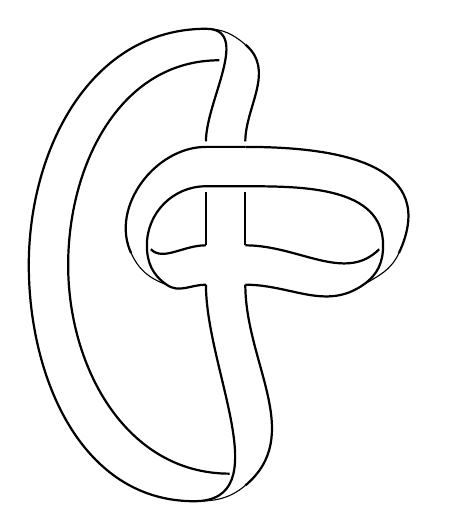
\begin{tikzpicture}
%centre coordinates
\coordinate (topl) at (-0.25,0.25); \coordinate (topr) at (0.25, 0.25);, \coordinate (botl) at (-0.25, -0.25); \coordinate (botr) at (0.25,-0.25);

%horizontal band coords
\coordinate (hleftt) at (-1, 0.25); \coordinate (hleftb) at (-0.75,-0.25); \coordinate (hleftm) at (-1.2, 0.15);
\coordinate (hrightt) at (2, 0.25); \coordinate (hrightb) at (1.75, -0.25); \coordinate (hrightm) at (2.2, 0.15); \coordinate (hrightx) at (2, 1);

%vertical band coords
\coordinate (vcrossbl) at (-0.25, 1); \coordinate (vcrosstl) at (-0.25, 1.5);
\coordinate (vcrossbr) at (0.25, 1); \coordinate (vcrosstr) at (0.25, 1.5);
\coordinate (vtopl) at (-0.25,3); \coordinate (vtopr) at (0.25, 2.8); \coordinate (vtopm) at (-0.08,2.6);
\coordinate (vleftl) at (-2.5, 0); \coordinate (vleftr) at (-2, 0);
\coordinate (vbotl) at (-0.4,-3); \coordinate (vbotr) at (0.25, -2.8); \coordinate (vbotm) at (0.05,-2.65);

%horizontal band draw
\draw [thick, shorten >=2] (topl) to [out=180, in=-45] (hleftt);
\draw [thick] (hleftm) to [out=115, in=180] (vcrosstl) to [out=0, in=180] (vcrosstr);
\draw [thick, distance=35] (vcrosstr) to [out=0, in=65] (hrightm);
\draw [thick, shorten <=2] (hrightt) to [out=-135, in=0] (topr);
\draw [thin] (hleftb) to [out=160, in=-65] (hleftm);
\draw [thin] (hrightb) to [out=30, in=-115] (hrightm);
\draw [thick] (botl) to [out=180, in=-35] (hleftb) to [out=145, in=-90] (hleftt) to [out=90, in=180] (vcrossbl) to [out=0, in=180] (vcrossbr) to [out=0, in=90] (hrightt) to [out=-90, in=35] (hrightb) to [out=-145, in=0] (botr);

%vertical band draw
\draw [thick, shorten >=2] (topl) to [out=90, in=-90] (vcrossbl);
\draw [thick, shorten <=2] (vcrosstl) to [out=90, in=0] (vtopl) to [out=180, in=90] (vleftl) to [out=-90, in=180] (vbotl) to [out=0, in=-90] (botl);

\draw [thick, shorten >=2] (topr) to [out=90, in=-90] (vcrossbr);
\draw [thick, shorten <=2] (vcrosstr) to [out=90, in=-40] (vtopr);
\draw [thick] (vtopm) to [out=180, in=90] (vleftr) to [out=-90, in=180] (vbotm);
\draw [thick] (vbotr) to [out=40, in=-90] (botr);
\draw [thin] (vtopr) to [out=140, in=0] (vtopl);
\draw [thin] (vbotr) to [out=-140, in=0] (vbotl);

\end{tikzpicture}
\caption{The torus with puncture maximally deformed.}
\end{figure}


\begin{figure}
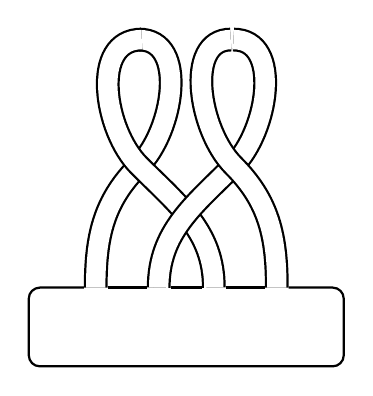
\begin{tikzpicture}[scale=2]
%'disc' coordinates
\coordinate (topl) at (-1,0); \coordinate (topr) at (1,0); \coordinate (botl) at (-1,-0.5); \coordinate (botr) at (1, -0.5);
\coordinate (breakl1) at (-0.65,0); \coordinate (breakl2) at (-0.5,0); \coordinate (breakml1) at (-0.25,0); \coordinate (breakml2) at (-0.1,0); \coordinate (breakmr1) at (0.1,0); \coordinate (breakmr2) at (0.25,0); \coordinate (breakr1) at (0.5,0); \coordinate (breakr2) at (0.65,0);
%draw `disc'
\draw[thick, rounded corners] (breakl2) -- (breakml1);
\draw[thick, rounded corners] (breakml2) -- (breakmr1);
\draw[thick, rounded corners] (breakmr2) -- (breakr1); 
\draw[thick, rounded corners] (breakr2) -- (topr) -- (botr) -- (botl) -- (topl) -- (breakl1);

%band coords
\coordinate (breakmidl) at (-0.575,0); \coordinate (breakmidmr) at (0.175,0); \coordinate (breakmidml) at (-0.175,0); \coordinate (breakmidr) at (0.575,0);
\coordinate (leftmidb) at (-0.3,0.775);
\coordinate (leftmidt) at (-0.3,1.575);
\coordinate (rightmidb) at (0.3,0.775);
\coordinate (rightmidt) at (0.3,1.575);
%left band draw
\draw[thick, double distance=7pt] (breakmidl) to [out=90, in=-135] (leftmidb) to [out=45, in=0] (leftmidt);
\draw[thick, double distance=7pt, shorten <=-1] (leftmidt) to [out=180,in=135] (leftmidb) to [out=-45, in=90] (breakmidmr);
%right band draw
\draw[thick, double distance=7pt] (breakmidml) to [out=90, in=-135] (rightmidb) to [out=45, in=0] (rightmidt);
\draw[thick,double distance=7pt, shorten <=1] (rightmidt) to [out=180,in=135] (rightmidb) to [out=-45, in=90] (breakmidr);
\end{tikzpicture}
\caption{}
\end{figure}

\end{document}